\section{Spatial discretization}
%
BOUT++ comes with a built in set of spatial discretization operators.
The operators used in the CELMA code is given in \cref{tb:spatop}.
%
\begin{table}[h!]
{\footnotesize \centerline{
\begin{tabular}{c|lll}
\hline\hline
%
Direction & First derivative stencil ($\partial_i f$) & Second derivative stencil ($\partial^2_i f$)& Upwind stencil ($f \partial_i g$)\\
%
\hline
%
$\rho$  & Centered second order & Centered second order & None\\
$\theta$ & Fast fourier transform & Fast fourier transform & None\\
z  & Centered second order & Centered second order & First order upwinding\\
%
\hline\hline
\end{tabular}
}}
\caption[]{\textit{Spatial operators used in the CELMA code.}}
\protect\label{tb:spatop}
\end{table}
%
The standard centred finite difference stencils has been used (see \cite{Leveque2007book} for details).
The fast fourier transform is implemented using the \texttt{fftw}-package \cite{FFTW05}.
The following term has been implemented with the first order upwinding scheme
%
\begin{itemize}[noitemsep,nolistsep]
    \item $-u_{e,\|}\partial_\|\ln(n)$
    \item $-u_{i,\|}\partial_\|(n[u_{i,\|}+u_{e,\|}])$
    \item $2u_{e,\|}\partial_\|(nu_{e,\|})$
\end{itemize}
%
notice that whereas the upwinding makes the system more stable, it does so by introducing heavy damping on the system through diffusion introduced by the discretization \cite{Leveque2007book}.
For this reason, upwinding is \textbf{NOT} used on the $u_{i,\|}\partial_\|\Om$ term when using the Boussinesq approximation as this may introduce spurious vorticity from the numerics.

\section{Boundary conditions}
%
The boundaries ar positioned half between grid points, as depicted in \cref{fig:flatBC}.
%
\begin{figure}[htb]
    \centering
    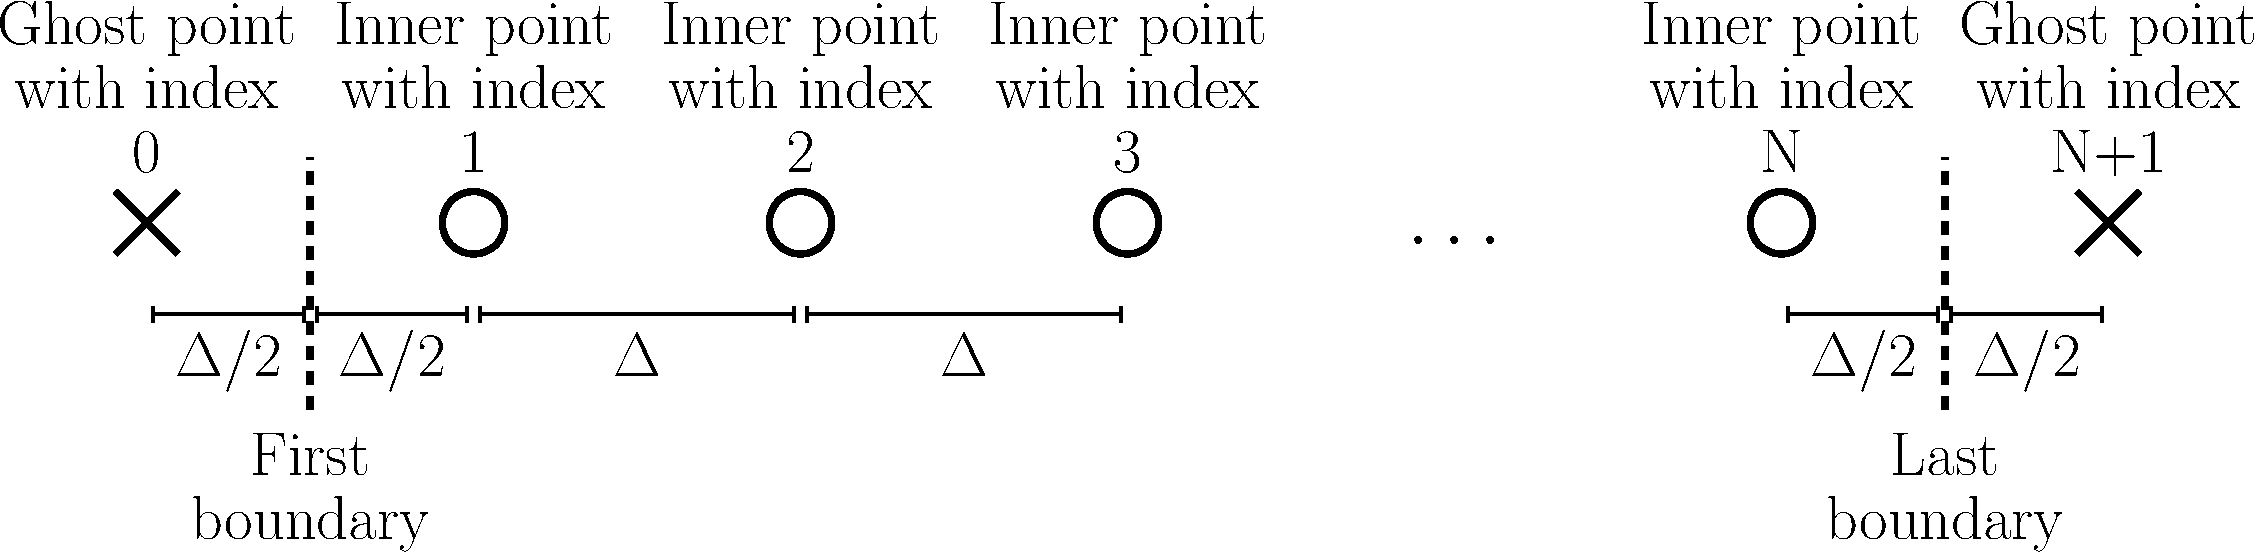
\includegraphics[width=1.0\textwidth]{fig/flatGrid}
    \caption{\textit{
            The boundaries ar positioned half between grid points.
            $\Delta$ denotes the grid spacing between two grid points.
        }}
    \label{fig:flatBC}
\end{figure}
%
The boundary condition given in \cref{fig:BCs} gives a value at the position of the boundary.
As there is no grid point at the boundary, the value is extrapolated to the ghost point $\frac{\Delta}{2}$.
For the Dirichlet boundary condition, the following $4$th order extrapolation %
%
\footnote{
Derived using a Newton polynomial (using the four points around the edge of the domain of \cref{fig:flatBC} (including the ghost point)), and evaluate it in the ghost point.
}%
is used
%
\begin{align*}
      f_{0} =& \frac{16}{5}f_{\text{First boundary}}
              - 3          f_1
              +            f_2
              - \frac{1}{5}f_3
    \\
      f_{N} =& \frac{16}{5}f_{\text{Last boundary}}
              - 3          f_{N}
              +            f_{N-1}
              - \frac{1}{5}f_{N-2}
\end{align*}
%
For the Neumann boundary condition a $4$th order extrapolation %
%
\footnote{
Derived using a one sided stencil (using the five points around the edge of the domain of \cref{fig:flatBC} (including the ghost point)) of the first derivate evaluated at the boundary, and solve for it for the ghost point.
% See D4DX4/BW2ndOrderNeumann4thOrder
}%
%
is used, reading
%
\begin{align*}
      f_0 =& \frac{12}{11}\Delta f_{\text{First boundary}}
                +
                \frac{
                  17f_1
                +  9f_2
                -  5f_3
                +   f_4
               }{22}
    \\
      f_{N+1} =& \frac{12}{11}\Delta f_{\text{Last boundary}}
                +
                \frac{
                  17f_{N}
                +  9f_{N-1}
                -  5f_{N-2}
                +   f_{N-3}
               }{22}
\end{align*}
%
In the cases where no boundary is imposed (for the parallel derivative of $\phi$ mentioned in \cref{sec:BCs} and in the composite derivatives mentioned in \cref{sec:compDeriv}), the following extrapolation %
%
\footnote{
Derived using a Newton polynomial (using the five points around the edge of the domain of \cref{fig:flatBC} (excluding the ghost point)), and evaluate it in the ghost point.
}%
is used for the ghost points
%
\begin{align}
    f_{N+1} =& 4f_{N} - 6f_{N-1} + 4f_{N-2} - f_{N-3},
    \label{eq:extraPolUp}
    \\
    f_{0} =& 4f_{1} - 6f_{2} + 4f_{3} - f_{4}
    \label{eq:extraPolDown}
\end{align}
%
Finally, as the $\theta$ direction is periodical, the ghost points are simply
%
\begin{align*}
    f_{N+1} =& f_{1}
    \\
    f_{0} =& f_{N}
\end{align*}
